\section{Experiments}
% \subsection{Reconstruction Comparison}
\subsection{Implementation Details}
\noindent\textbf{Datasets \& Preprocess.} Our model is trained on 4 panorama datasets, including one image dataset, Flickr360~\cite{cao2023ntire}, and three video datasets, WEB360~\cite{wang2024360dvd}, ODV360~\cite{cao2023ntire}, and 360+x~\cite{chen2024x360}.
%
Among them, only WEB360~\cite{wang2024360dvd} comes with captions; therefore, we use Qwen-VL~\cite{Qwen-VL} to annotate the remaining three datasets, generating corresponding descriptive captions.
%
All datasets are resized to a resolution of $512 \times 1024$, and during training, video data is divided into clips of 49 frames each.


\noindent\textbf{Training.} We first inflate the patch embedding layer of the powerful video generation model, Wan2.1~\cite{wan2025}, from 16 to 33 channels to accommodate the input data, and then fine-tune the entire model.
%
The training process is executed on 8 $\times$ NVIDIA A100 GPUs, using a batch size of 1 and a learning rate of $1e-4$. 
%
We employ a joint image-video training strategy, treating images as videos with only one frame.



%\noindent\textbf{Inference.}% Optional 
\begin{figure}[t]
  \centering
   \vspace{-0.5cm}
  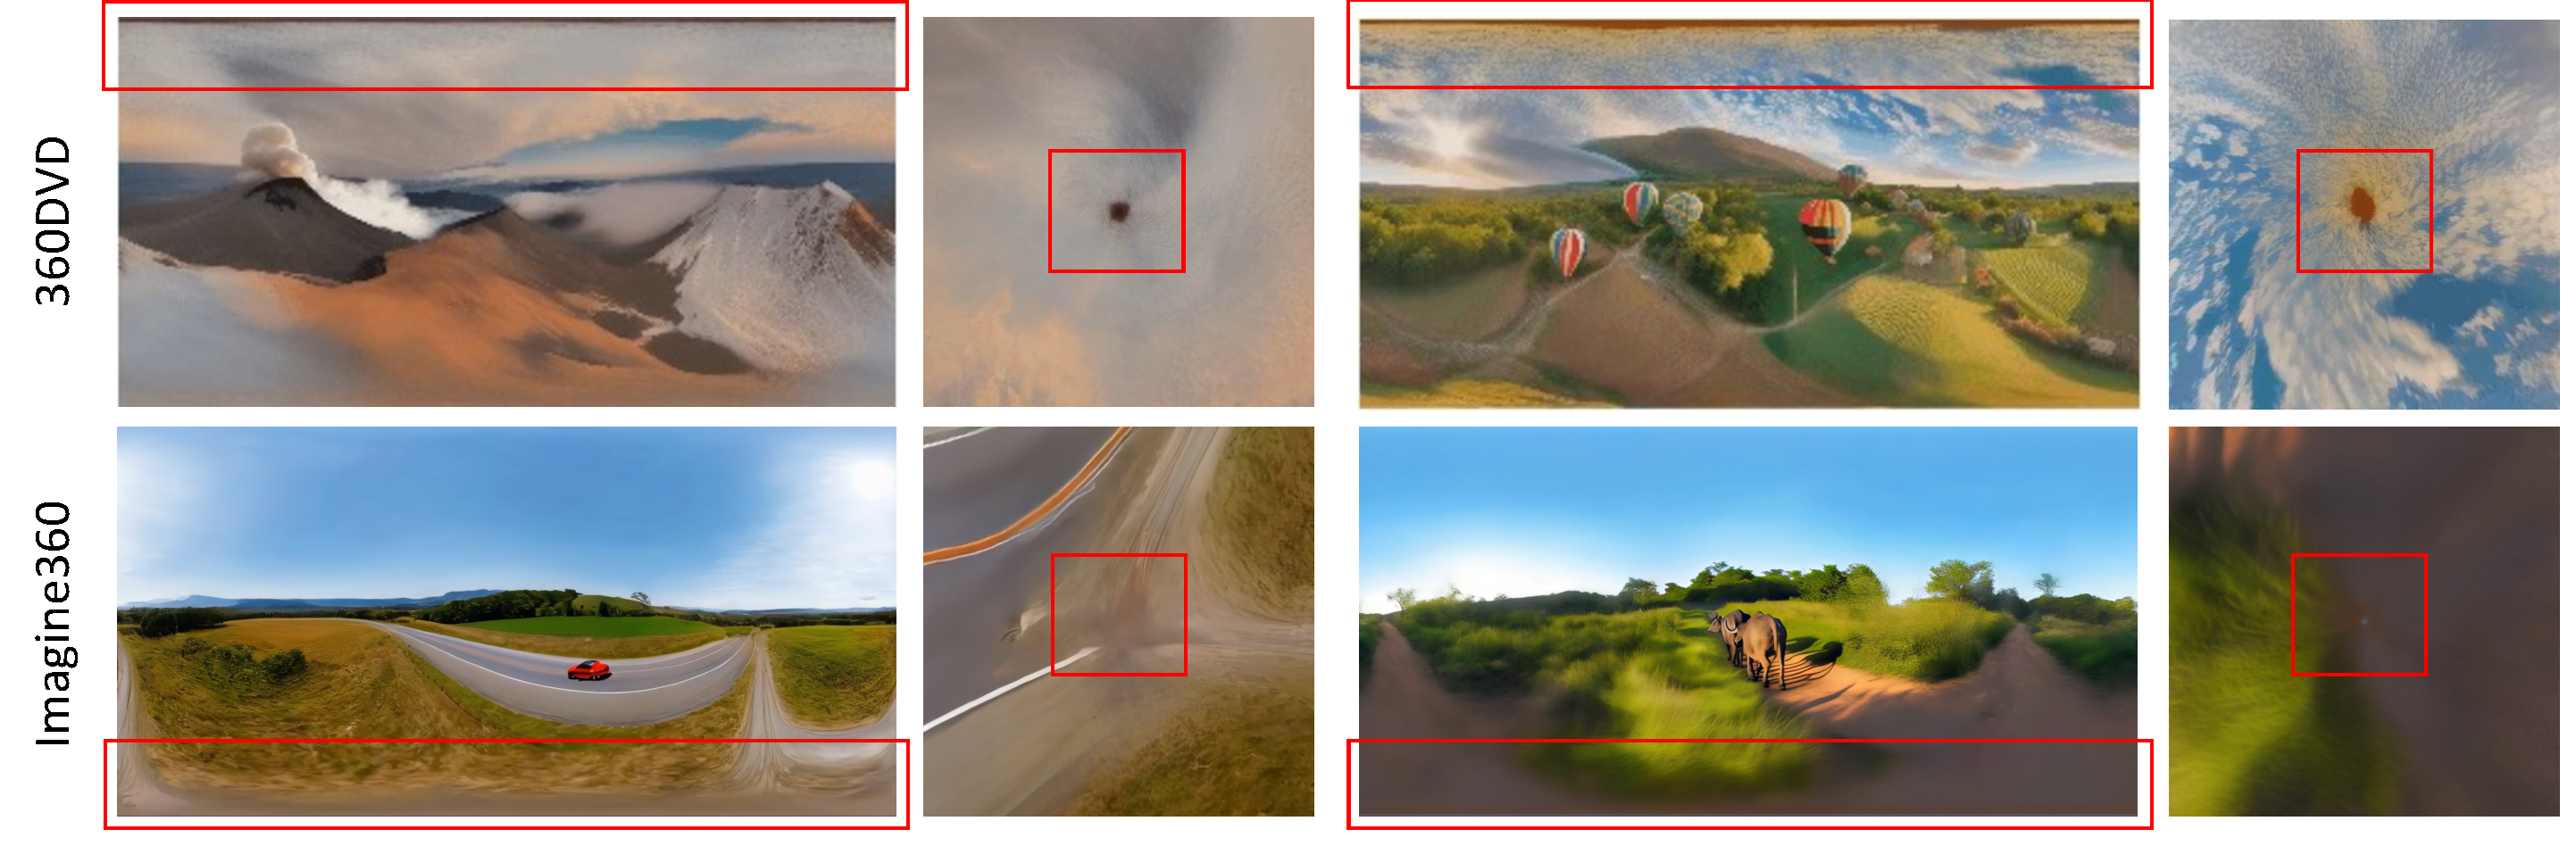
\includegraphics[width=1\linewidth]{figs/exp1.pdf}
  \caption{\textbf{Results from 360DVD~\cite{wang2024360dvd} and Imagine360~\cite{tan2024imagine360}.} Despite numerous efforts to mitigate geometric distortion at the poles, both methods still struggle with generating realistic top and bottom views. The distortion at the poles is even more pronounced in video scenes, severely affecting realism and immersion.}
  \label{fig:exp1}
  \vspace{-0.5cm}
\end{figure}
\subsection{Qualitative Comparison}
We compare our approach with three previous methods, including one perspective video outpainting method, Follow-Your-Canvas~\cite{chen2024follow}, and two 360-degree video generation methods, 360DVD~\cite{wang2024360dvd} and Imagine360~\cite{tan2024imagine360}. 
%
Adopting equirectangular representation, both 360DVD~\cite{wang2024360dvd} and Imagine360~\cite{tan2024imagine360} exhibit severe distortion at the poles.
%
As shown in~\cref{fig:exp1}, the sky appears to have ``black holes", while the ground shows ``swirls".
%
We argue that these artifacts are caused by the model's difficulty in handling the spatial-temporal distortion introduced by ERP, as a slight movement can result in significant disturbances at the poles.

The visualization of the comparison results is shown~\cref{fig:compare}, where we present the ERP format and perspective views in four horizontal directions, with arrows indicating the flow of time.
%
As shown in~\cref{fig:compare}, 360DVD~\cite{wang2024360dvd} only recognizes textual input. The generated frames exhibit terrible image quality and possess little motion.
%
Follow-Your-Canvas(F-Y-C)~\cite{chen2024follow} generates satisfactory perspective videos; however, its results suffer from severe spatial inconsistency, especially on the $\mathcal{B}$ face, exhibiting a noticeable sense of disconnection.
%
Although Imagine360~\cite{tan2024imagine360} synthesizes reasonable panoramic videos, it lacks spatial-temporal continuity.
%
As in the first example, the little girl is running, but the ground does not move accordingly and shows a noticeable texture difference from the input video.
%
In the second example, the aircraft in the input video is in a dark and tense atmosphere, while the generated panoramic video shows blue skies and white clouds, creating a peaceful scene. 
%
Additionally, the aircraft does not integrate well with the surrounding environment, resulting in a discordant effect.
%
In contrast, our approach demonstrates excellent spatial-temporal consistency and supports both textual prompts and input videos, thus enhancing the flexibility of generation. 
%
Furthermore, ViewPoint exhibits high motion dynamics, as each perspective view responds to the motion trends of the input video correctly.
%
As in the first case, the input video depicts a little girl running forward, with the prompt describing a magical forest scene at night. 
%
Our generated video aligns with both the input video and the prompt, showcasing a strong capability for condition awareness and integration.
%
Similarly, in the second example, the generated panoramic video also integrates with the input video and exhibits high-quality dynamics.
\begin{figure}[t]
  \centering
   \vspace{-0.5cm}
  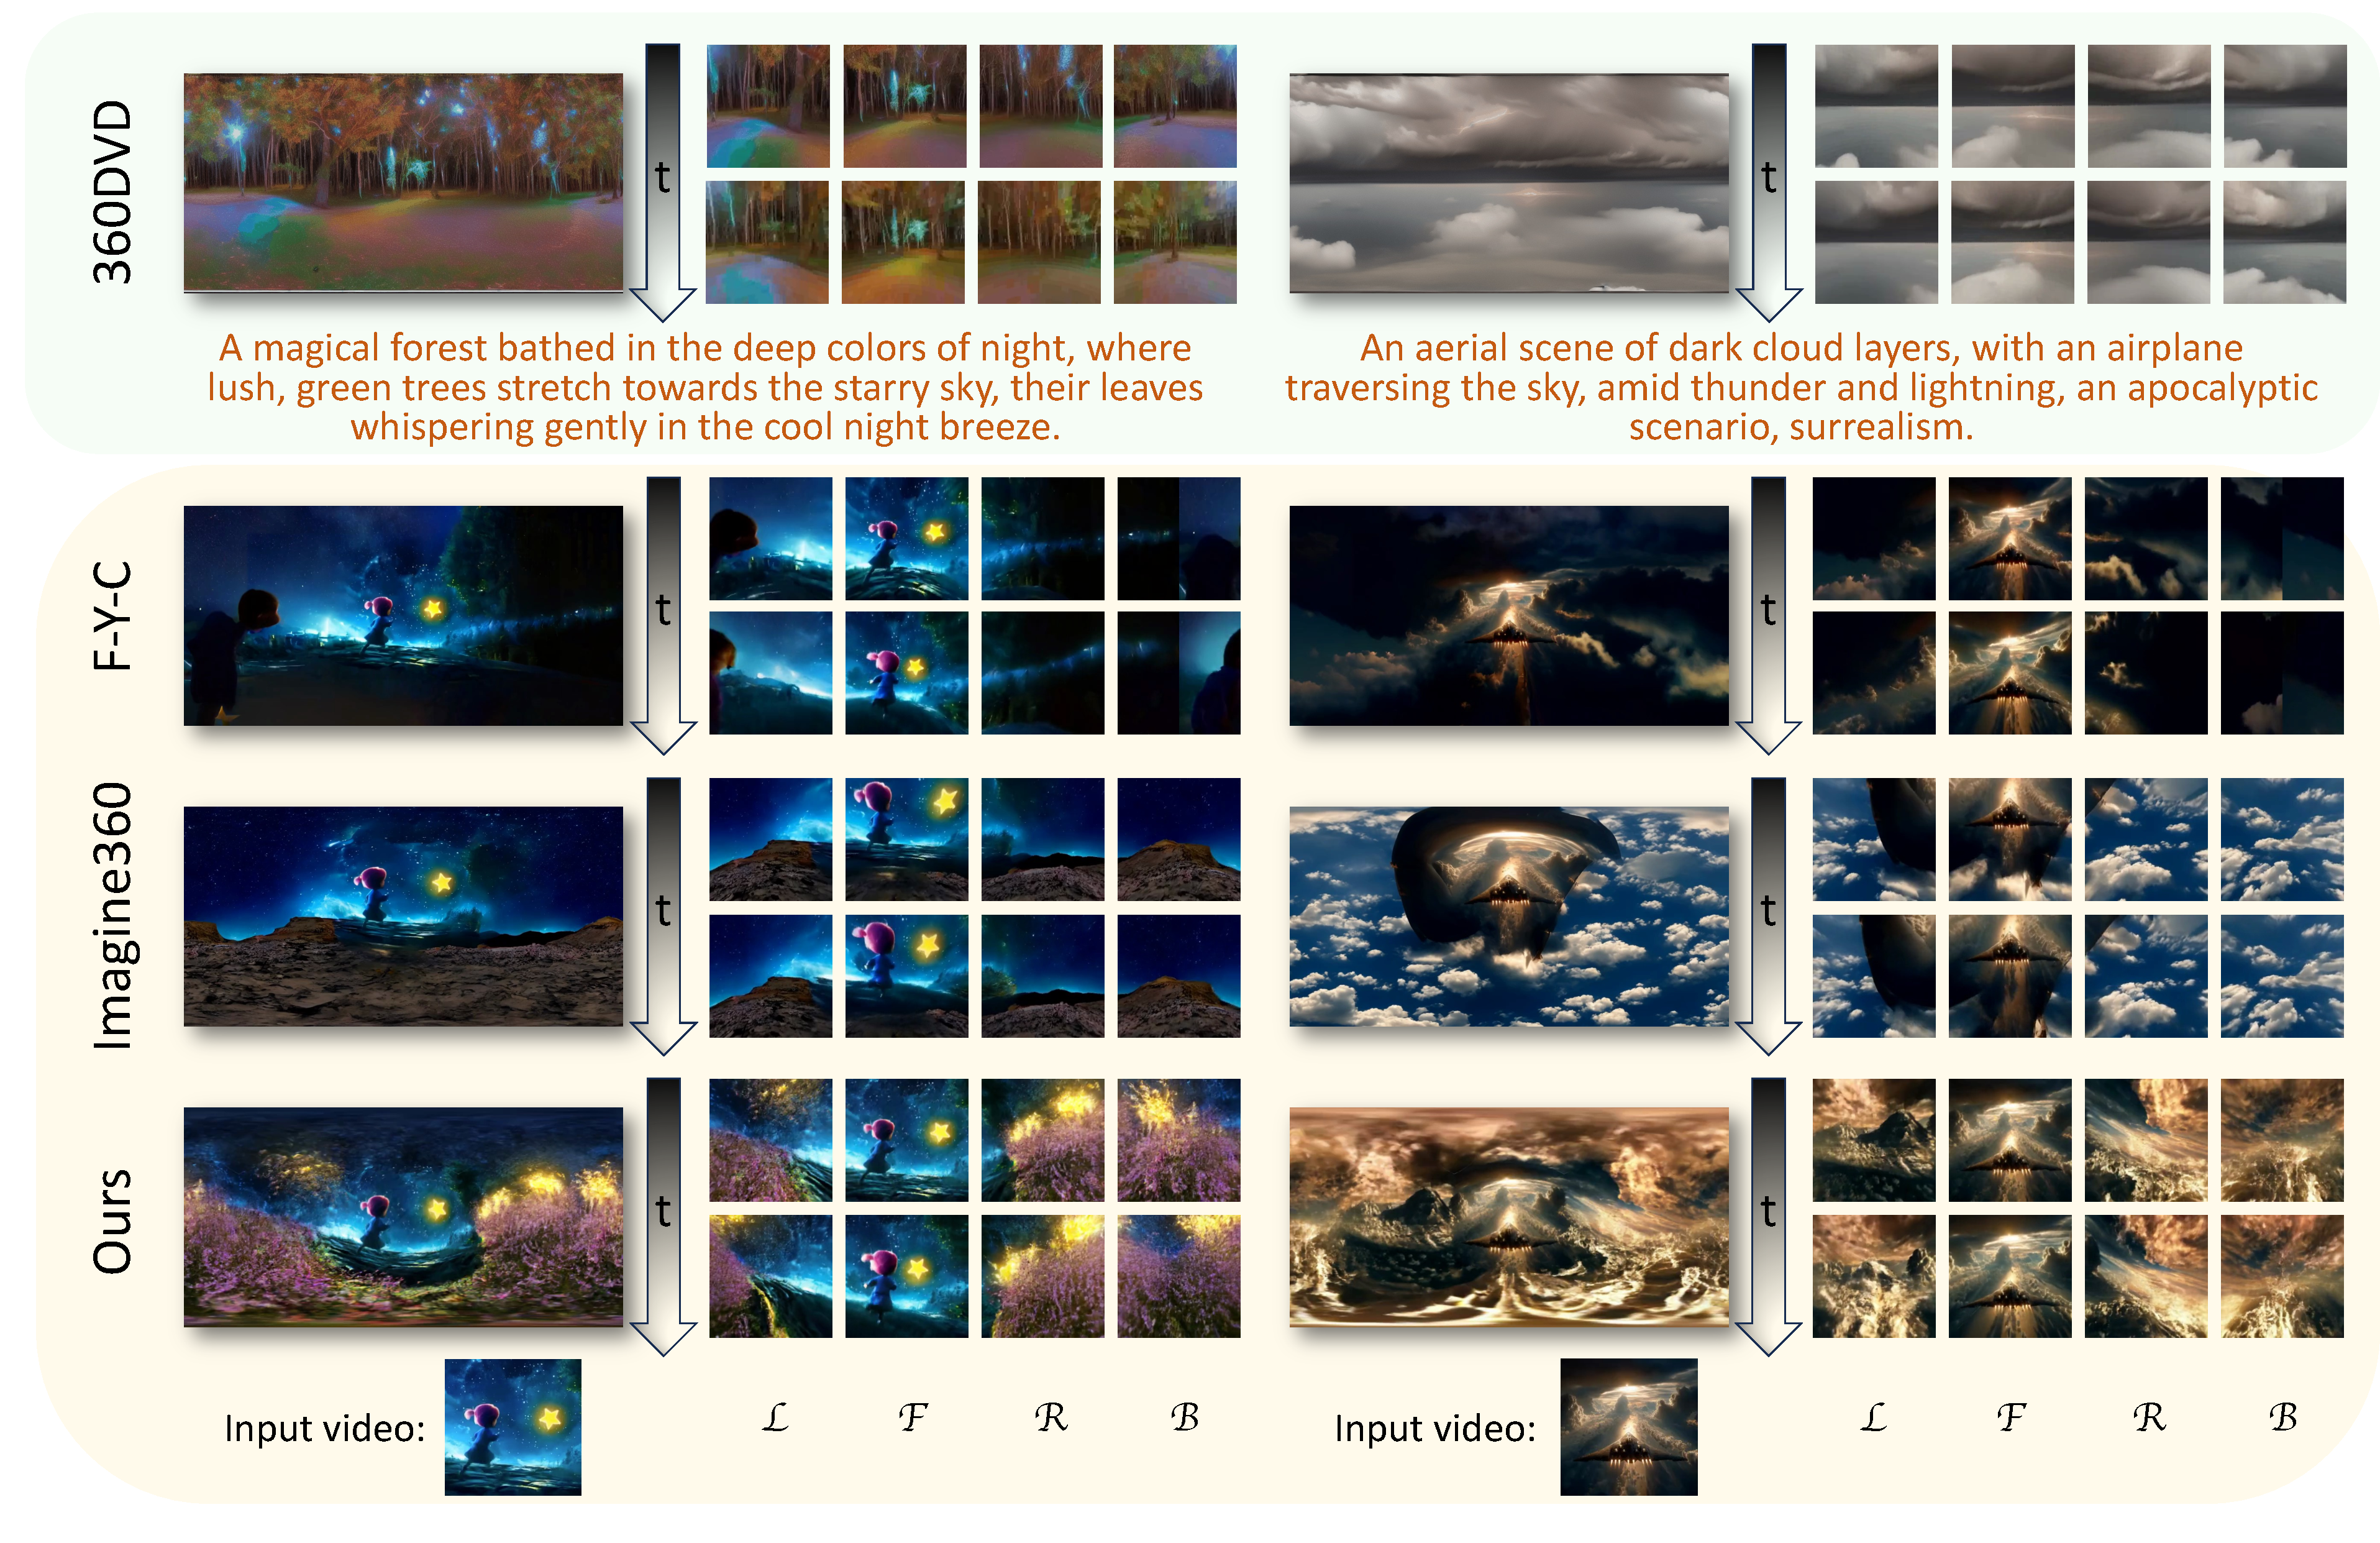
\includegraphics[width=1\linewidth]{figs/compare.pdf}
  \caption{\textbf{Qualitative comparison of generated videos.} 360DVD is a text-driven approach and exhibits terrible image quality while Follow-Your-Canvas fails to generate panoramic videos with a reasonable spatial layout. Imagine360 suffers from spatial-temporal discontinuity. Our approach, on the other hand, can generate high-quality panoramic videos aligned with the given input. Due to page limits, we highly recommend watching the dynamic videos available at \href{https://becauseimbatman0.github.io/ViewPoint}{\textcolor{red}{ViewPoint}}.}
  \label{fig:compare}
  %\vspace{-0.5cm}
\end{figure}

\subsection{Quantitative Comparison}
In this section, we provide a quantitative comparison of our approach with previous methods. 
%
VBench~\cite{huang2023vbench} is a comprehensive benchmark suite for video generative models which scores a video in 16 dimensions.
%
We evaluate our approach and previous methods on the ODV360~\cite{cao2023ntire} dataset across five dimensions: ``subject consistency", ``imaging quality", ``motion smoothness" and ``dynamic degree".
%
Specifically, we first project the generated videos into six perspective views with a FoV of 90$^\circ$, similar to $\mathcal{F,R,B,L,U,}$ and $\mathcal{D}$.
%
Then, we apply VBench~\cite{huang2023vbench} evaluation in a perspective manner for all projected videos.
%

The results of the quantitative evaluation are shown in~\cref{tab:vbench}, where our approach achieves the best scores across four metrics.
%
Although 360DVD~\cite{wang2024360dvd} performs the second best in ``subject consistency", it scores the lowest in ``dynamic degree", indicating that the videos generated by 360DVD have very little motion. 
%
The nearly static videos result in 360DVD achieving a high score in ``motion smoothness"; however, such videos fail to meet the demands of generating high-quality panoramic videos. 
%
Follow-Your-Canvas~\cite{chen2024follow}, on the other hand, is capable of generating high-quality perspective results, but the projected videos exhibit severe spatial distortion, resulting in poor performance in evaluations.
%
In contrast, our approach demonstrates state-of-the-art performance in all four metrics, proving that our method can generate highly dynamic and temporally coherent panoramic videos.

% \begin{table}[h]
% \setlength\tabcolsep{2pt}%
% \renewcommand\arraystretch{1.2}

%   \centering
%   % \vspace{-2mm}
%     \caption{\textbf{Quantitative comparison on VBench.} Our method achieves the best performance in four metrics and the second place in one metric. Although 360DVD obtains the second highest ``subject consistency" score due to the nearly static nature of its generated videos, the results fail to meet the demands of generating high-quality panoramic videos. In contrast, our approach performs well in both motion consistency and dynamics.}
%     % \vspace{2mm}
    
%     \resizebox{1\linewidth}{!}{
%    \begin{tabular}{c|ccccc}
%     \toprule
%     Method  & subject consistency$\uparrow$ & imaging quality$\uparrow$ & motion smoothness$\uparrow$ & aesthetic quality$\uparrow$ & dynamic degree$\uparrow$ \\
%     \midrule
%     Follow-Your-Canvas~\cite{chen2024follow} &0.8284 &0.4464 &0.9655 &0.4118 &0.8500 \\
%     360DVD~\cite{wang2024360dvd}  &0.8633 &0.5394 &0.9703  &0.4651 &0.5083\\
%     Imagine360~\cite{tan2024imagine360}  &0.8547 &0.5859 &0.9720  &\textbf{0.5313} &0.8148 \\
    
%     \textbf{\method(Ours)}  &\textbf{0.8793} &\textbf{0.5927} &\textbf{0.9800} &0.5052 &\textbf{0.9083}\\
%     \bottomrule
%   \end{tabular}
% }
%   \label{tab:vbench}
% \end{table}

\begin{table}[h]
\setlength\tabcolsep{2pt}%
\renewcommand\arraystretch{1.2}

  \centering
  % \vspace{-2mm}
    \caption{\textbf{Quantitative comparison on VBench.} Our method achieves the best performance in all four metrics. Although 360DVD obtains the second highest ``subject consistency" score due to the nearly static nature of its generated videos, the results fail to meet the demands of generating high-quality panoramic videos. In contrast, our approach performs well in both motion consistency and dynamics.}
    % \vspace{2mm}
    
    \resizebox{0.8\linewidth}{!}{
   \begin{tabular}{c|cccc}
    \toprule
    Method  & subject consistency$\uparrow$ & imaging quality$\uparrow$ & motion smoothness$\uparrow$ & dynamic degree$\uparrow$ \\
    \midrule
    Follow-Your-Canvas~\cite{chen2024follow} &0.8284 &0.4464 &0.9655  &0.8500 \\
    360DVD~\cite{wang2024360dvd}  &0.8633 &0.5394 &0.9703   &0.5083\\
    Imagine360~\cite{tan2024imagine360}  &0.8547 &0.5859 &0.9720  &0.8148 \\
    
    \textbf{\method(Ours)}  &\textbf{0.8793} &\textbf{0.5927} &\textbf{0.9800} &\textbf{0.9083}\\
    \bottomrule
  \end{tabular}
}
  \label{tab:vbench}
\end{table}

\subsection{Ablation Study}
To demonstrate the effectiveness of our method, we conduct ablation experiments on panorama representation formats and network designs.
%
For the ERP format, we directly fine-tune the base model to adapt to this panoramic representation. 
%
For the CP format, we train two models, CP-ICLoRA and CP-4DRoPE, separately to assess the impact of different cubeface-encodings.
%
Technically, CP-ICLoRA rearranges the six cube faces into a 2-row by 3-column rectangle in raster order, \ie $\mathcal{F,R,B}$ on the first row, and $\mathcal{L,U,D}$ on the second row, while CP-4DRoPE assigns an independent positional encoding to each cube face.
%
We also examine the design of Pano-Perspective attention by replacing all Perspective blocks with the intact Pano blocks.

As shown in~\cref{fig:ablation}, ERP exhibits significant artifacts due to the inherent modality gap with the pretrained model. 
%
Both cubemap representation methods suffer from spatial discontinuity, wherein CP-4DRoPE shows inconsistency in color tone, while CP-ICLoRA, although achieving better image quality, presents significant spatial fractures.
%
Our full method, in contrast, is capable of generating high-quality and coherent panoramic videos that are superior to other alternative designs in both spatial and temporal aspects.

The results of quantitative ablation are shown in~\cref{tab:ablation}, our full method outperforms the other four alternative designs across four metrics.
%
Since we conduct evaluations in a perspective manner, CP-ICLoRA performs best in ``imaging quality''. However, as shown in~\cref{fig:ablation}, though each perspective video shows good visual quality, there is still a discontinuity issue at the boundaries of the cube faces. 

\begin{figure}[t]
  \centering
    \vspace{-0.5cm}
  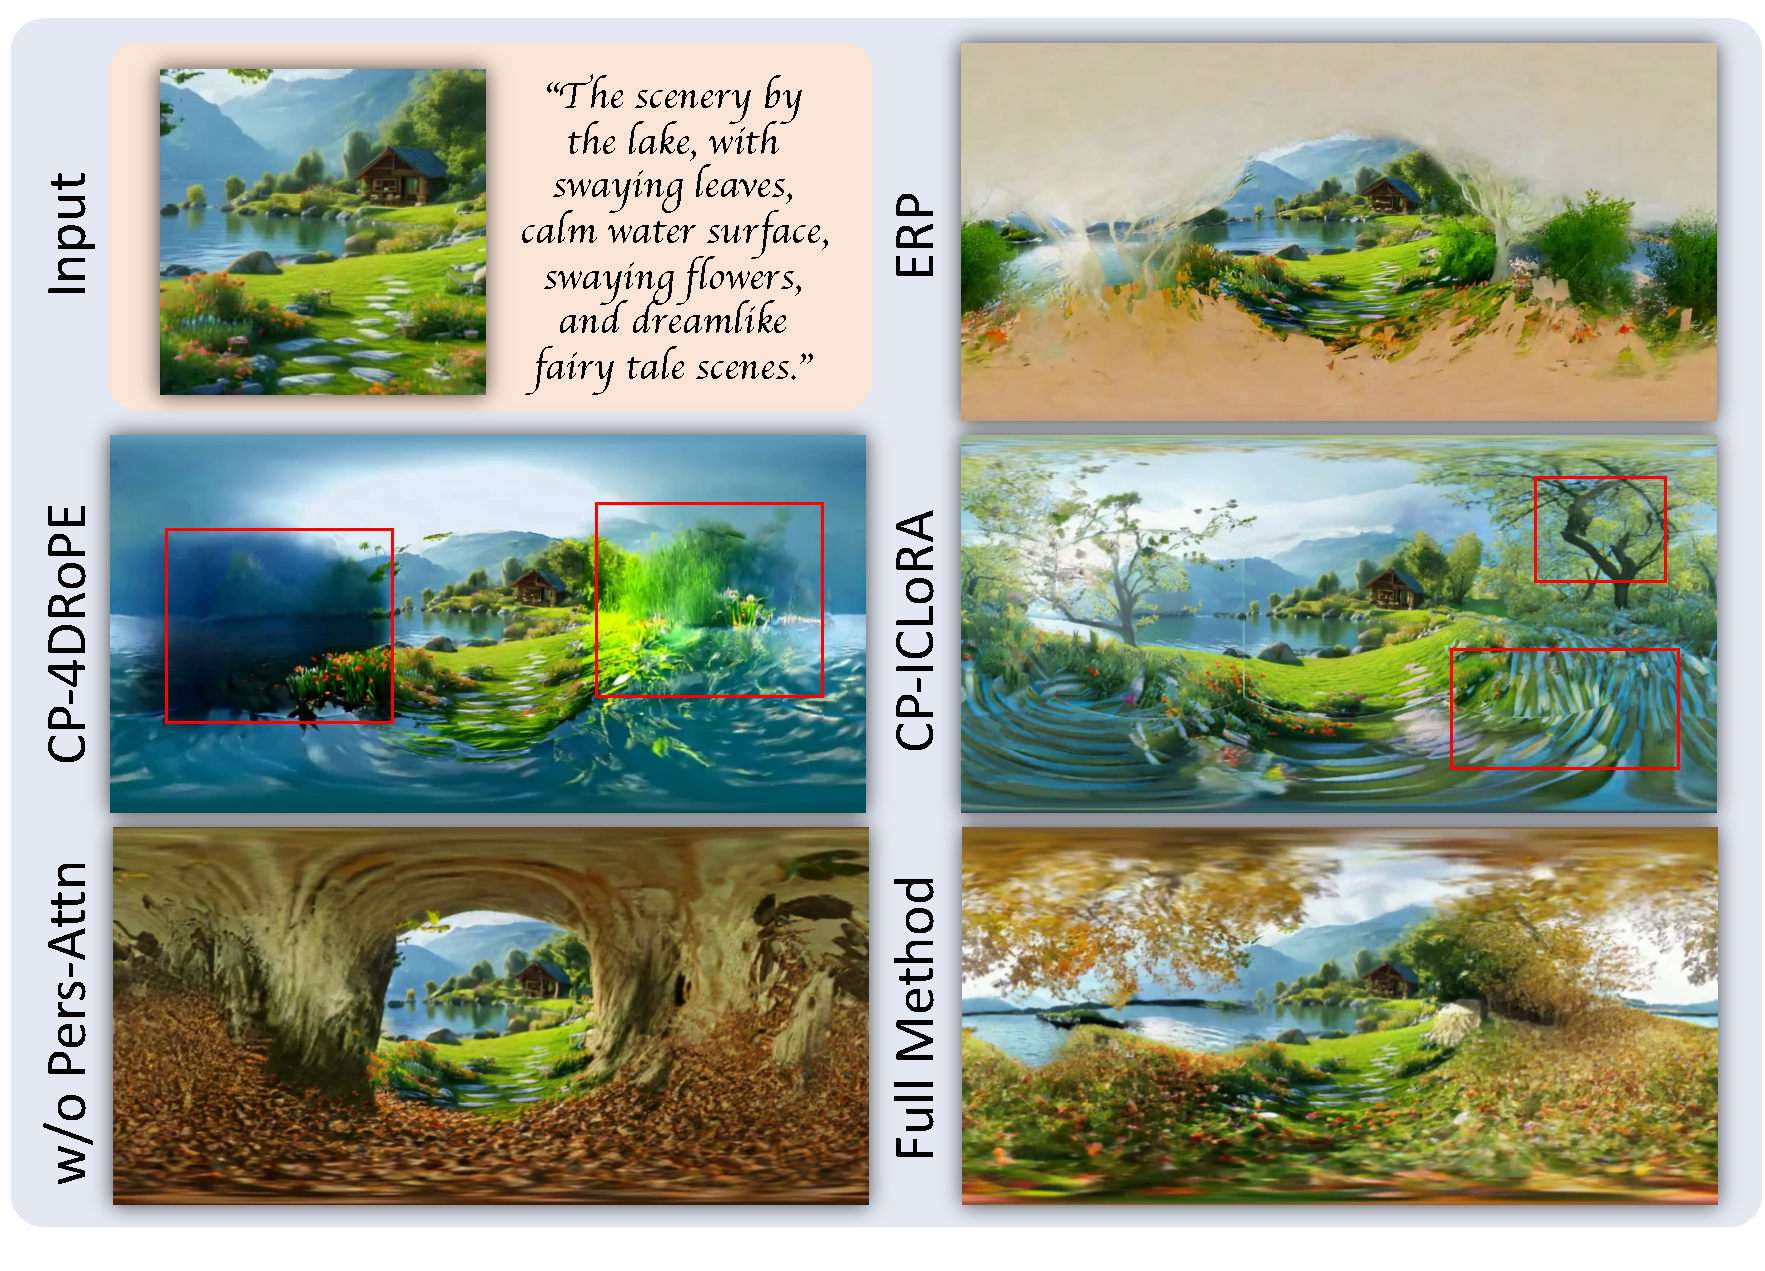
\includegraphics[width=1\linewidth]{figs/ablation.pdf}
   \vspace{-8.0mm}
  \caption{\textbf{Ablation on different designs.} ERP exhibits serious artifacts due to the natural gap in modality. Both Cube representation methods have spatial discontinuity issues. Without Perspective-Attention, it leads to misalignment with the input video. Our full method can generate reasonable and spatially consistent results.}
  \label{fig:ablation}
  \vspace{-5.5mm}
\end{figure}

% \begin{table}[h]
% \setlength\tabcolsep{2pt}%
% \renewcommand\arraystretch{1.2}

%   \centering
%   % \vspace{-2mm}
%     \caption{\textbf{Quantitative ablation.} Compared to the other four alternative designs, our approach achieves the highest scores across four metrics.}
%     % \vspace{2mm}
    
%     \resizebox{1\linewidth}{!}{
%    \begin{tabular}{c|ccccc}
%     \toprule
%        & subject consistency$\uparrow$ & imaging quality$\uparrow$ & motion smoothness$\uparrow$ & aesthetic quality$\uparrow$ & dynamic degree$\uparrow$ \\
%     \midrule
%     ERP &0.8702 &0.5396 &0.9781 &0.4913 &0.8840\\
%     CP-4DRoPE  &0.8612 &0.5104 &0.9633  &0.5012 &0.8175  \\
%     CP-ICLoRA  &0.8727 &\textbf{0.6018} &0.9786  &0.4930 &0.8946  \\
%     w/o Perspective-Attn  &0.8663 &0.5392 &0.9798  &0.4254 &0.8827 \\
%     \textbf{Full Method}  &\textbf{0.8793} &0.5927 &\textbf{0.9800} &\textbf{0.5052} &\textbf{0.9083} \\
%     \bottomrule
%   \end{tabular}
% }
%   \label{tab:ablation}
% \end{table}
\begin{table}[h]
\setlength\tabcolsep{2pt}%
\renewcommand\arraystretch{1.2}

  \centering
  % \vspace{-2mm}
    \caption{\textbf{Quantitative ablation.} Compared to the other four alternative designs, our approach achieves the highest scores across three metrics. Although CP-ICLoRA achieves the highest score in ``imaging quality", proving that each of the six faces has good quality independently, the panoramas composed of these six faces exhibit noticeable discontinuities, as indicated by the red boxes in~\cref{fig:ablation}. Therefore, it does not meet the demand for high-quality panoramic video generation.}
    % \vspace{2mm}
    
    \resizebox{0.8\linewidth}{!}{
   \begin{tabular}{c|ccccc}
    \toprule
       & subject consistency$\uparrow$ & imaging quality$\uparrow$ & motion smoothness$\uparrow$ & dynamic degree$\uparrow$ \\
    \midrule
    ERP &0.8702 &0.5396 &0.9781 &0.8840\\
    CP-4DRoPE  &0.8612 &0.5104 &0.9633  &0.8175  \\
    CP-ICLoRA  &0.8727 &\textbf{0.6018} &0.9786   &0.8946  \\
    w/o Perspective-Attn  &0.8663 &0.5392 &0.9798  &0.8827 \\
    \textbf{Full Method}  &\textbf{0.8793} &0.5927 &\textbf{0.9800}  &\textbf{0.9083} \\
    \bottomrule
  \end{tabular}
}
  \label{tab:ablation}
\end{table}
\subsection{User Study}
Despite achieving advanced scores on VBench~\cite{huang2023vbench}, we conduct user studies, introducing subjective user ratings to further validate the superiority of our approach.
%
We ask participants to vote on the tested videos based on four dimensions: ``Spatial Continuity", ``Temporal Quality", ``Aesthetic Preference" and ``Condition Alignment". ``Spatial continuity" represents the coherence of scenes and structures in panoramic space, while ``Temporal Quality" is used to evaluate motion effects; for example, being nearly motionless and flickering are considered poor performance. ``Aesthetic Preference" represents participants' subjective preferences, while ``Condition Alignment" refers to the degree to which the generated panoramic video aligns with the input conditions, such as text or video.
%
% \begin{wrapfigure}{r}{0.5\linewidth}
%     % \vspace{-2.5mm}
%     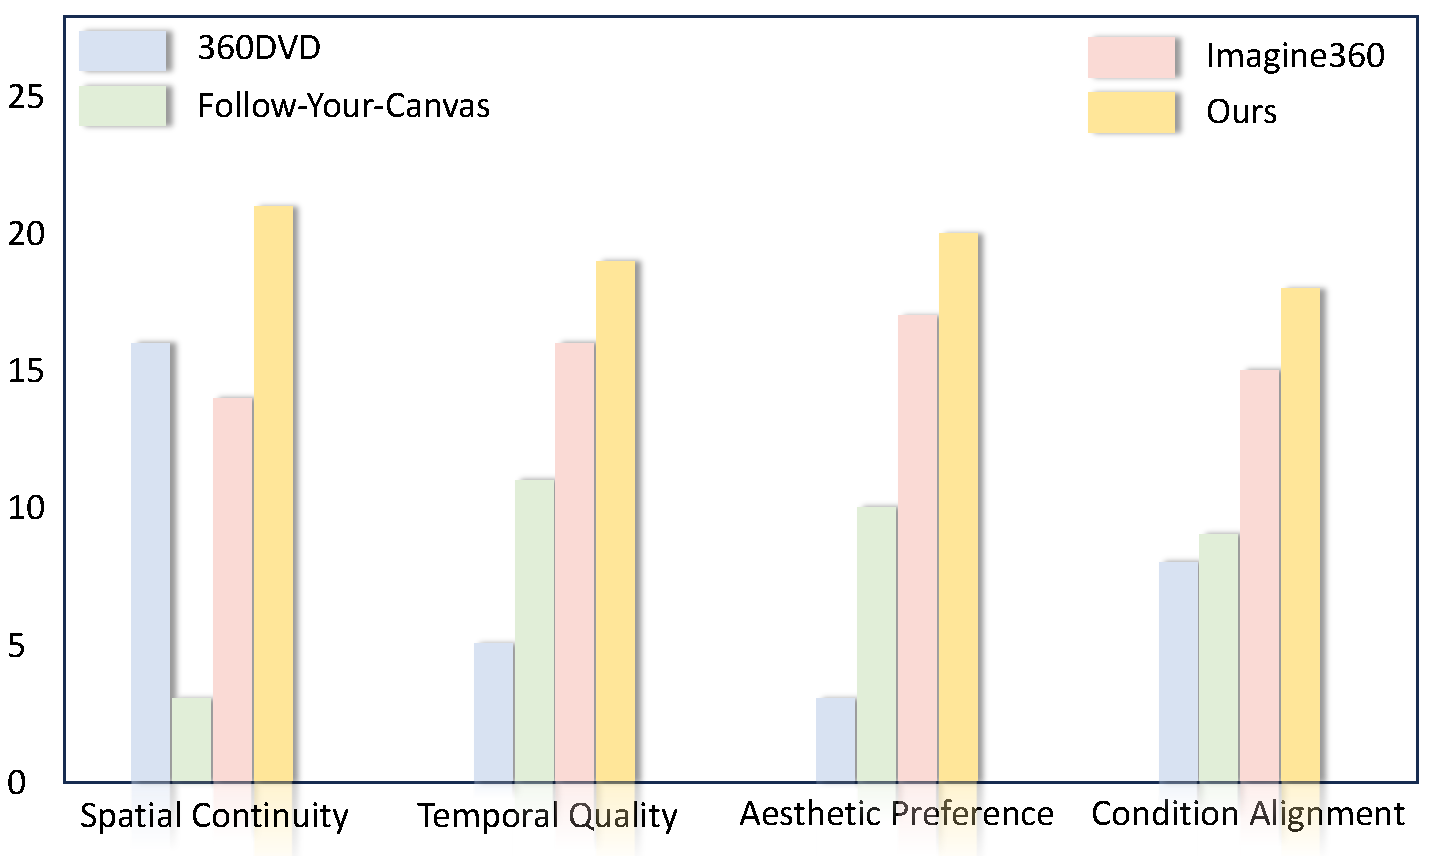
\includegraphics[width=0.9\linewidth]{figs/user.pdf}
%     \caption{\textbf{User studies.} We ask participants to vote on the videos generated by four methods based on four dimensions, and our approach receives the most votes.}
%      % \vspace{-15.0mm}
%     \label{fig:user}
% \end{wrapfigure}

Finally, we collect 50 valid questionnaires, each containing 14 sets of videos for comparison, and the results are shown in~\cref{fig:user}.
%
Overall, Imagine360~\cite{tan2024imagine360} is the second choice among participants, while 360DVD~\cite{wang2024360dvd} and Follow-Your-Canvas~\cite{chen2024follow}, receive the fewest votes.
%
Our approach receives the highest number of votes across all four dimensions, surpassing 360DVD~\cite{wang2024360dvd}, Follow-Your-Canvas~\cite{chen2024follow}, and Imagine360~\cite{tan2024imagine360}, demonstrating our method's ability to generate satisfactory panoramic results.
%


% \begin{figure}[h]
%   \centering
%     % \vspace{-1.0cm}
%   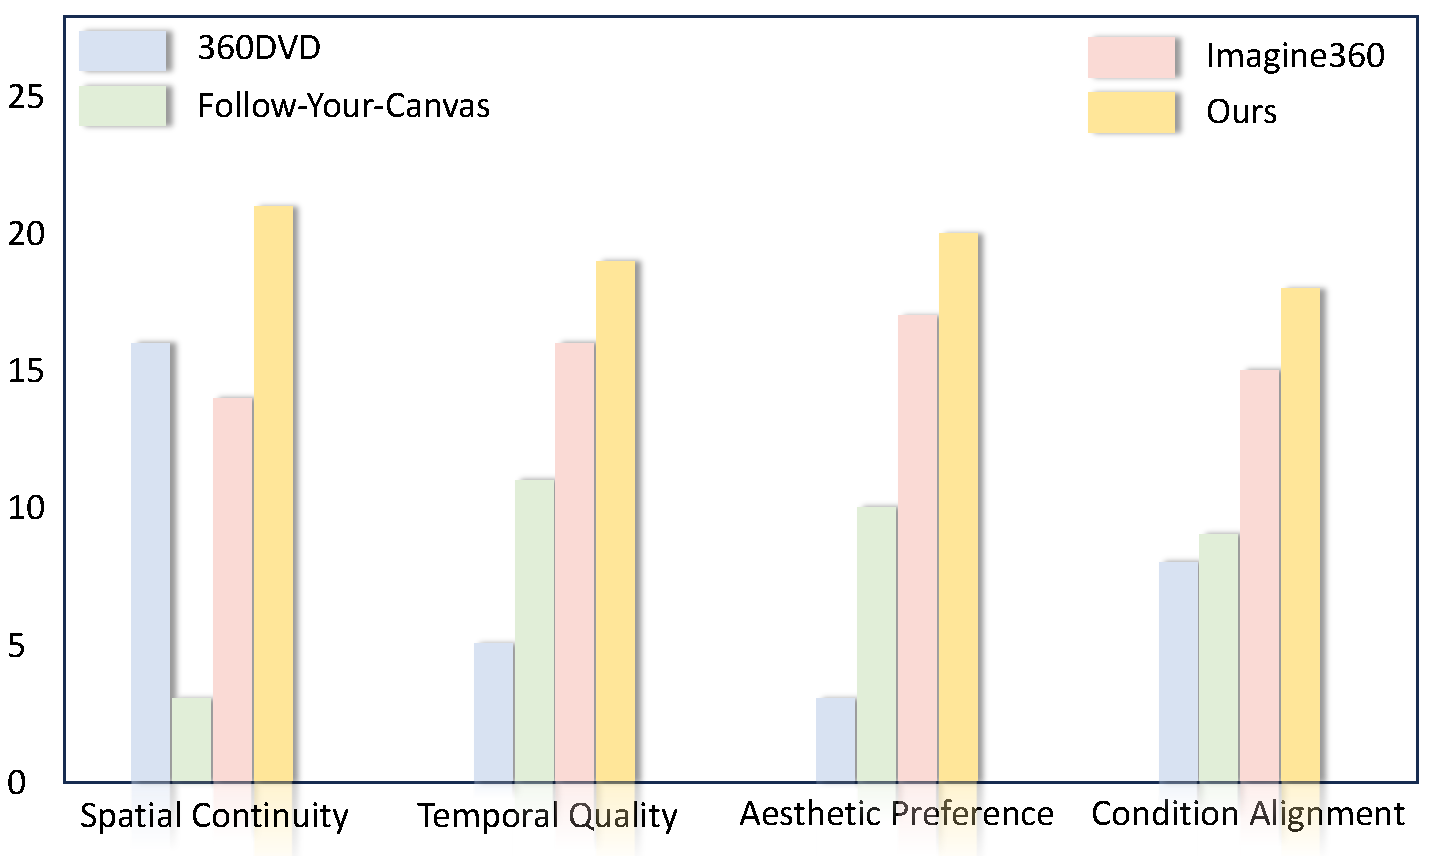
\includegraphics[width=0.6\linewidth]{figs/user.pdf}
%   \caption{\textbf{User studies.} We ask participants to vote on the videos generated by four methods based on four dimensions, and our approach receives the most votes.}
%   \label{fig:user}
%   %\vspace{-0.5cm}
% \end{figure}